\begin{frame}
	\frametitle{Adaptive Sampling: Theory}
	 \begin{columns}[onlytextwidth,T]
      \column{\dimexpr\linewidth-6cm-5mm}
        
        Adaptive sampling takes advantage of surrogate information content \textit{during training} to reduce sample quantity.\newline
        
        We developed a technique which is novel in the literature:
        \begin{itemize}
        \item Construct surrogate quality distribution by nearest- neighbour interpolation.
        \item Draw candidate samples by quality using MCMC.
        \item Include samples with high crowding distance.
        \item Repeat!
        \end{itemize}
      \column{6cm}
      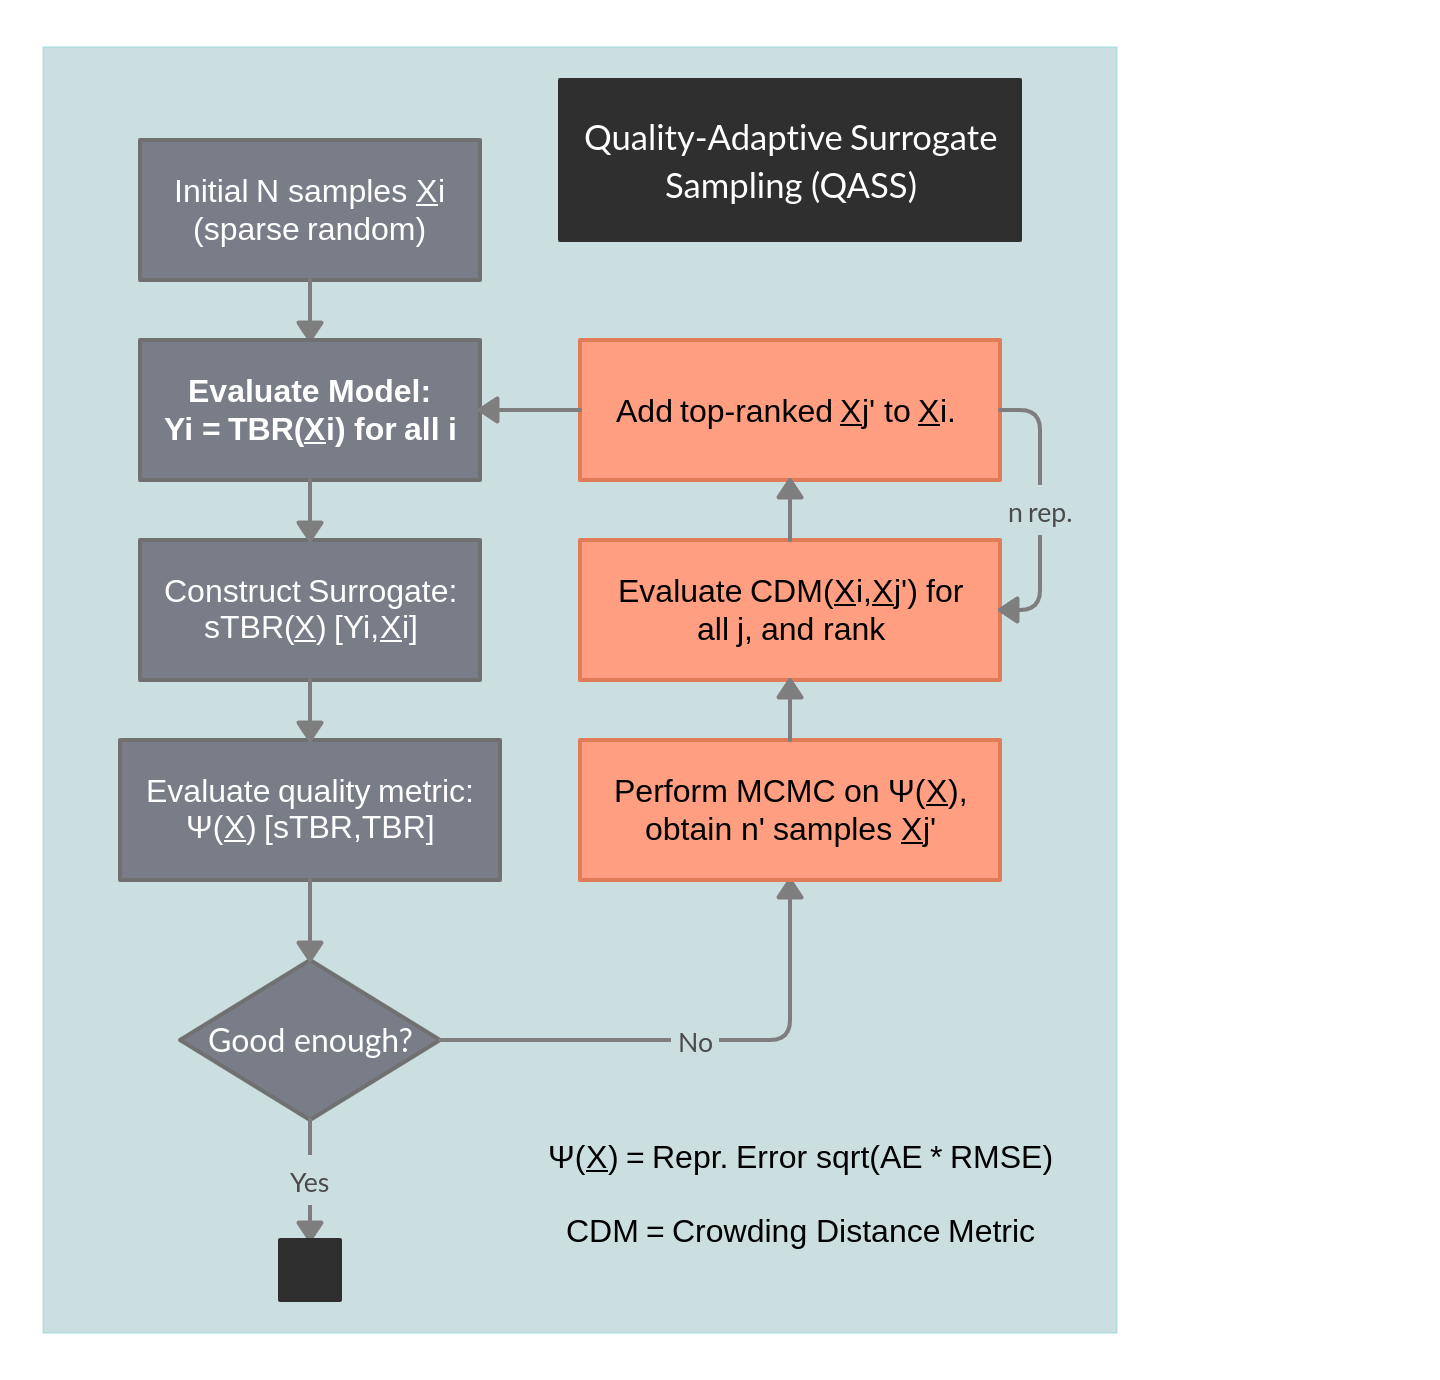
\includegraphics[width=8cm]{qassplan}

    \end{columns}
\end{frame}

\begin{frame}
	\frametitle{Application on Toy Theory}
	\begin{itemize}
		\item % TODO
	\end{itemize}
\end{frame}
